\documentclass[12pt,a4paper,fleqn]{article}
\usepackage{rmpackages}																% usual packages
\usepackage{rmtemplate}																% graphic charter
\usepackage{rmexocptce}																% for DS with cptce eval
\usepackage{multirow}

%\cfoot{} 													% if no page number is needed
%\renewcommand\arraystretch{1.5}		% stretch table line height

\begin{document}
\normalem

\begin{header}
TP -- Gaston ne manque pas d'air !
\end{header}

\begin{multicols}{2}
\begin{center}
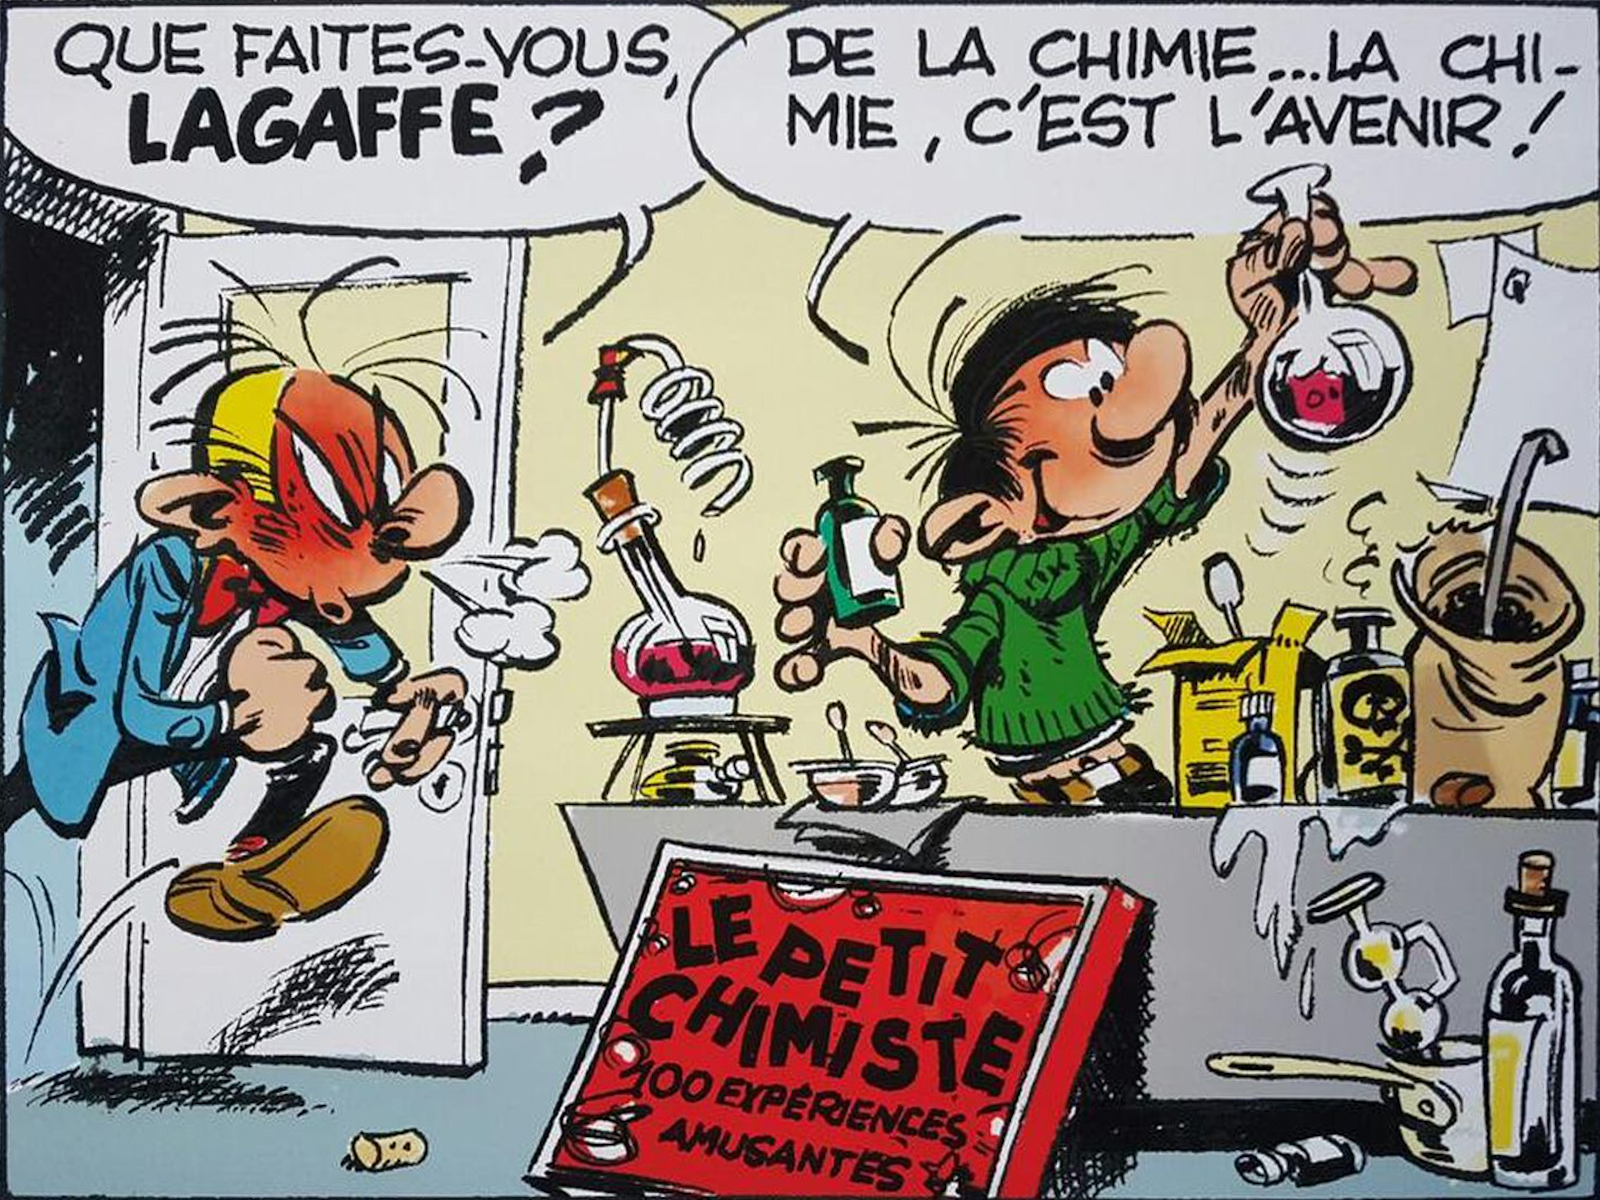
\includegraphics[width=\linewidth]{images/lagaffe.png}
\end{center}

\hfill

Pour impressionner mademoiselle Jeanne sans trop se fatiguer, Gaston a encore eu une idée de génie : gonfler un ballon aussi gros que possible avec la réaction chimique entre le vinaigre et le bicarbonate de soude.

Malheureusement, il n'a que \qty{2,5}{\gram} de bicarbonate de soude et désire utiliser un minimum de vinaigre : le reste servira pour l'entretien de son vieux tacot.
Il a besoin de votre aide !
\end{multicols}

\begin{doc}
\label{doc:co2}
\textbf{Production de gaz}

Le vinaigre est une solution aqueuse d'acide éthanoïque, de formule $\mathrm{C_2O_2H_4}$.
Il réagit avec l'hydrogénocarbonate de sodium, de formule $\mathrm{NaHCO_3}$, selon l'équation de réaction
\[
\mathrm{C_2O_2H_4 + NaHCO_3 \rightarrow NaC_2O_2H_3 + H_2O + CO_2.}
\]
\end{doc}

\begin{doc}
\textbf{Réactif limitant}

Une réaction chimique ne se déroule pas éternellement.
Lorsqu'au moins un des réactifs est entièrement consommé, la réaction s'arrête : ce réactif s'appelle le \textbf{réactif limitant}.

Si tous les réactifs sont entièrement consommés, on dit qu'ils ont été mélangés dans des proportions \textbf{stœchiométriques}.
À la fin de la réaction, il n'y a plus de réactif. 
\end{doc}

\begin{multicols}{2}
\begin{doc}
\label{doc:manip}
\textbf{Manipulation}

\begin{enumerate}
\item Peser \qty{2,5}{g} de bicarbonate de soude, puis les verser dans un ballon de baudruche à l'aide d'un entonnoir.
\item Prélever un volume $V_\mathrm{vinaigre}$ de vinaigre, puis le verser dans un erlenmeyer.
\item Ajouter trois gouttes de BBT.
\item Boucher l'erlenmeyer avec le ballon sans verser le bicarbonate.
\item \label{quest:manip} Une fois que l'erlenmeyer est \textbf{hermétiquement fermé}, verser \textbf{doucement} le bicarbonate dans le vinaigre.
\end{enumerate}
\end{doc}

\begin{doc}
\textbf{Le BBT}

Le bleu de bromothymol (BBT) est un \textbf{indicateur coloré}.
Il prend une teinte :
\begin{itemize}
\item \textcolor{yellow_f}{jaune} si la solution est \textbf{acide} ;
\item \textcolor{bleu_f}{bleue} si la solution est \textbf{basique} ;
\item \textcolor{green_f}{verte} si la solution est \textbf{neutre}.
\end{itemize}

Ici, un excès d'acide éthanoïque rend la solution acide, tandis qu'un excès d'hydrogénocarbonate de sodium rend la solution basique.
La solution est plutôt neutre quand elle ne contient ni l'un ni l'autre.
\end{doc}

\end{multicols}

\section*{Gonfler le plus gros ballon avec un minimum de vinaigre}

\begin{enumerate}
\item \app{}

Identifier les réactifs et les produits de la réaction entre le vinaigre et le bicarbonate de soude.

\item \rea{}
Réaliser la manipulation décrite dans le document~\ref{doc:manip}.

\emph{Appeler le professeur avant de passer à la dernière étape !}
\end{enumerate}

\begin{appel}
\rea{}
\end{appel}

\begin{enumerate}[resume]
\item \rea{}

Compléter le tableau ci-dessous.

\item \rea{}

Schématiser l'expérience réalisée lors de l'étape~\ref{quest:manip} en utilisant le schéma narratif.

\item \app{} \val{} \com{}

Indiquer le volume minimal de vinaigre que Gaston doit utiliser pour obtenir le plus gros ballon possible.
Justifier en utilisant les termes suivants : \emph{stœchiométrique}, \emph{réactif limitant}.
\end{enumerate}
\begin{appel}
\com{}
\end{appel}

\begin{enumerate}[resume]
\item \rco{}

Nommer le gaz formé.
Quel test caractéristique permettrait de le mettre en évidence ?

\item \anarai{}

Vérifier que l'équation de la réaction du document~\ref{doc:co2} est bien \textbf{équilibrée}.
\thumbsup

\item \val{}

Quelle verrerie aurait-on pu utiliser pour mesurer \emph{précisément} le volume de vinaigre $V_\mathrm{vinaigre}$ ?

\end{enumerate}

\begin{center}
\renewcommand\arraystretch{1.5}		% stretch table line height
\begin{tabular}{|*{2}{>{\centering}p{.09\linewidth}|} *{4}{>{\centering\arraybackslash}p{.13\linewidth}|} >{\centering\arraybackslash}p{.07\linewidth}|}
\hline
\textbf{Groupe} & $V_\mathrm{vinaigre}$ (\unit{\milli\litre}) & \textbf{Teinte de la solution} & \textbf{Reste-t-il de l'acide ?} & \textbf{Reste-t-il du solide ?} & \textbf{Réactif limitant} & \textbf{$R_\mathrm{ballon}$ (\unit{cm})} \\
\hline \hline
\textbf{1} & \num{5,0} & & & & & \\
\hline
\textbf{2} & \num{10} & & & & & \\
\hline
\textbf{3} & \num{15} & & & & & \\
\hline
\textbf{4} &\num{20}  & & & & & \\
\hline
\textbf{5} & \num{25} & & & & & \\
\hline
\textbf{6} & \num{30} & & & & & \\
\hline
\textbf{7} & \num{35} & & & & & \\
\hline
\textbf{8} & \num{40} & & & & & \\
\hline
\textbf{9} & \num{45} & & & & & \\
\hline
\end{tabular}
\end{center}

\section*{Avec la quantité de matière}

En faisant ces tests, on a finalement utilisé beaucoup de vinaigre !
Aurait-on pu déterminer le volume minimal de vinaigre à utiliser sans en \og gaspiller \fg{} ?

Bien sûr !
Pour cela on va compter les particules qui réagissent en utilisant la mole.

\begin{enumerate}[resume]
\item \rea{}

Calculer le nombre $N_1$ de \og molécules \fg{} d'hydrogénocarbonate de sodium dans la quantité utilisée pour l'expérience.
\thumbsup

\item \rea{}

Calculer la quantité de matière $n_1$ d'hydrogénocarbonate de sodium utilisée pour l'expérience.

\item \anarai{}

Déterminer la quantité de matière $n_2$ d'acide éthanoïque à ajouter pour obtenir un mélange stœchiométrique.
\thumbsup

\item \rea{}
 
Calculer le volume d'acide éthanoïque à prélever.

\item \val{}

Les résultats expérimentaux sont-ils en accord avec vos calculs ?
\end{enumerate}

\begin{appel}
\val{}
\end{appel}

\paragraph{Données :}
\begin{itemize}
\item Masse d'une \og molécule \fg{} d'hydrogénocarbonate de sodium : $m_\mathrm{NaHCO_3} = \qty{1.39e-22}{g}$ ;
\item Constante d'Avogadro : $N_\mathrm{A} = \qty[per-mode=power]{6,022e23}{\per\mole}$ ;
\item La quantité de matière $n$ d'un échantillon contenant $N$ particules est donnée par $n=\frac{N}{N_\mathrm{A}}$ ;
\item \qty{100}{mL} du vinaigre utilisé contiennent \qty{0,133}{\mole} d'acide éthanoïque.
\end{itemize}

\end{document}